\documentclass{sig-alt-release2}

\usepackage{amssymb}
\setcounter{tocdepth}{3}
\usepackage{graphicx}
\usepackage{url}
\usepackage{subfigure}

%%%%%%%%%%%Añadido de CPB para controlar las versiones%%%%%%%
%Macros par los cambios
\usepackage[usenames]{color}
%\usepackage[dvips]{color}
\usepackage{colordvi}
\usepackage{ulem}
\normalem
\definecolor{MyDarkGreen}{rgb}{0,0.8,0.0}
\definecolor{MyDarkBlue}{rgb}{0,0,0.8}
\definecolor{MyDarkRed}{rgb}{0.6,0,0.0}
\newcommand{\borrar}[1]{\textcolor{MyDarkRed}{\sout{#1}}} %\sout}
\newcommand{\nuevo}[1]{\textcolor{MyDarkBlue}{\uline{#1}}} %\sout}
\newcommand{\nota}[1]{\textcolor{MyDarkGreen}{#1}} %\sout}
%%%%%%%%%%%%%%%%%%%%%%%%%%%%%%%%%%%%%%%%%%%%%%%%%%%%%%%%%%%%%%%%

\urldef{\mailsa}\path|cicamargoba@unal.edu.co|
\urldef{\mailsb}\path|cesarpedraza@usantotomas.edu.co|
% \newcommand{\keywords}[1]{\par\addvspace\baselineskip
% \noindent\keywordname\enspace\ignorespaces#1}

\begin{document}
\conferenceinfo{GECCO'11,} {July 12--16, 2011, Dublin, Ireland.}
\CopyrightYear{2011}
\crdata{978-1-4503-0690-4/11/07}
\clubpenalty=10000
\widowpenalty = 10000
\conferenceinfo{GECCO 2011}{2011 Genetic and Evolutionary Computation Conference}


% \mainmatter  % start of an individual contribution

% first the title is needed
\title{Intrinsic Evolvable Hardware for Combinatorial Synthesis Based on SoC+FPGA and GPU Platforms}

\numberofauthors{2}

\author{
\alignauthor Artificial Life, Robotics, Evolvable Hardware
% \alignauthor Carlos Camargo Bare\~{n}o\\
%        \affaddr{Universidad Nacional de Colombia}\\
%        \email{cicamargoba@unal.edu.co}
% \alignauthor C\'esar Pedraza\\
%        \affaddr{Universidad Santo Tom�s de Aquino}\\
%        \email{cesarpedraza@usantotomas.edu.co}
}

%\authorrunning{Short form of author list} % if too long for running head


% the affiliations are given next; don't give your e-mail address
% unless you accept that it will be published
% \institute{Universidad Nacional de Colombia. \\  Facultad de Ingenier\'ia, Bogot\'a Colombia \\
% Universidad Santo Tom\'as \\  Facultad de Ingenier\'a de Telecomunicaciones, Bogot\'a Colombia \\
% \mailsa, \mailsb\\
% }

\maketitle

\begin{abstract}
This paper presents a novel a parallel genetic programming (PGP) boolean synthesis implementation on a low cost cluster of an embedded platform called SIE, based on a 32-bit processor and a Spartan-3 FPGA. Some tasks of the PGP have been accelerated through a hardware coprocessor called FCU, that allows to evaluate individuals onchip as intrinsic evolution. Results have been compared with GPU and HPC implementations, resulting in speedup values up to approximately 2 and 180 respectively.  
\end{abstract}

\begin{keywords}
Evolutionary algorithms, boolean synthesis, cluster.
\end{keywords}
\section{Introduction.}

As an alternative to the traditional design of combinatorial circuits, some authors have proposed bio-inspired techniques to create combinatorial circuits that can not be obtained with the traditional methods and to add some restrictions to the design such as delay, area, etc, \cite{Nicholson, Kajitani:1996p16, Aguirre:2009p66, coello2000}. 
One of the main problems to create circuits by using these techniques is the response time, due the high computational requirements for implementing any bio-inspired algorithm. In order to use parallel genetic programming (PGP), an FPGA cluster-based architecture to solve the combinatorial synthesis problem on-chip has been developed. A fitness coprocessor unit (FCU) on each FPGA helps to accelerate the convergence of the algorithm, as well as provide an appropriate support for 12-variable synthesis problems, by evaluating a chromosome through a virtual LUT-oriented architecture without using high-latency partial reconfiguration techniques, and determining the fitness value for an individual faster than other related works. The proposed synthesis algorithm was compared to a High Performance Cluster (HPC) and a graphics processing unit (GPU) implementations. 
For this work a tree based representation for circuits was selected. Basic cells can construct any circuit, each composed by 3 functions $f$ and 4 input variables $v$ coded in binary in 28 bits. The chromosome length has to be variable because the length of the solution to the synthesis problem is unknown a priori.
In equation \ref{fitness} the fitness function for the proposed genetic program (GP) is shown. Constants $\omega_{1}$, $\omega_{2}$ and $\omega_{3}$ are used for establishing the weights of each of the parameters that will determine the fitness function. The double-summation term calculates the number of matches of the individual X for all the possible combinations at the output with the target functions Y; the $P(X)$ function is used for calculating the number of logic gates of a chromosome taking into account some of the $introns$ or segments of the genotype string that will not have any associated function and that do not contribute to the result of the logic circuit that they represent. The function $L(X)$ is used for determining the number of levels the circuit has, or in other words the number of gates that the critical path crosses. The $m$ constant is the number of outputs in the circuit and $n$ the number of possible combinations of inputs in the circuit.

\begin{equation}
\label{fitness}
fitness=\omega_{1} . [ \sum_{j=1}^m \sum_{i=1}^n Y(j,i)-X(j,i) ] + \omega_{2}.P(x) + \omega_{3}.L(x)
\end{equation}

A selection operator is responsible for identifying the best individuals of the population taking into account the exploitation and the exploration \cite{QYCC06}. The first one allows the individuals with better fitness to survive and reproduce more often, and the second one means searching in more areas and making it possible to find better results. In the other hand, the mutation operator modifies the chromosome randomly in order to increase the search space. It can change: 1) an operator or variable and 2) a segment in the chromosome. A one or two points crossover operator combines two selected individuals for obtaining two additional individuals to add to the population. 


% &&&&&&&&&&&&&&&&&&&&&&&&&&&&&&&&&&&&&&&&&&&&&&&&&&&&&&&&&&&&&&&&&&&&&&&&&&&&&&&&&&&&&&&&&&&&&&&&&&&&
%                                                                     PROGRAMACION GENETICA 
% &&&&&&&&&&&&&&&&&&&&&&&&&&&&&&&&&&&&&&&&&&&&&&&&&&&&&&&&&&&&&&&&&&&&&&&&&&&&&&&&&&&&&&&&&&&&&&&&&&&&

\section{GP Implementation.}
\textbf{HPC and SIE:} The GP was implemented in a small-low-cost FPGA-based cluster platform called SIE, a Graphics Processing Unit (GPU) and a High Performance Computer (HPC) called ALTAMIRA. SIE \cite{WSCC} created by our team work, is composed of a custom embeddded platform and a software development kit based on Linux operating system, and provides an economical alternative (70 USD per node) for implementing evolutionary algorithms. In contrast, other authors use architectures for implementing similar applications, closed to 1000 USD y 3000 USD per node \cite{JJPR, ZVLS07} 

The GP was implemented in two stages: the first one is about software development and its parallelization on HPC and GPUs, and the second one refers to a hardware implementation to speed it up on the SIE plataform.
Using the island approach, the population is divided into sub-populations that will evolve in each processor of the cluster or parallel architecture, making data migration to accelerate convergence. 

\textbf{GPU: }
In the GPU platform a function called $kernel-GP$ is executed on each processing element that evolves a sub-population of the GP. Additionally, a  Mersenne-twister algorithm is executed on the GPU before the $kernel-GP$ to make a buffer of random numbers on its own global memory (figure \ref{fig:migration_scheme}) shows the way the GP has been implemented on the graphics device. A thread $t$ generates a $\mu$-population, performs the GP operators during $P$ generations required. $M$ best individuals will be transferred to the global memory and then to the host device (CPU system).

\begin{figure}[htpb]
\begin{center} 

\includegraphics[width=7cm]{./images/migration_scheme} \end{center}
\caption{GPU implementation of the evolvable algorithm.}\label{fig:migration_scheme}
\end{figure}

A profiling determined that the most costs were the fitness function calculation and the new individual generation. They have been accelerated with a dedicated hardware in the FPGA (FCU). Inside (figure \ref{fig:hw_block}), the chromosome cells are converted to an equivalent Virtual Look Up Table (VLUT) with a ROM based translation, in order to calculate of wrong minterms compared to the objective function. Also, the FCU calculates the final fitness value including the number of gates and the critical path. In order to speed up pseudo random number generation, a Mersenne-Twister-based coprocessor was inserted through the same custom interface. 

\begin{figure}[htpb]
\begin{center} 
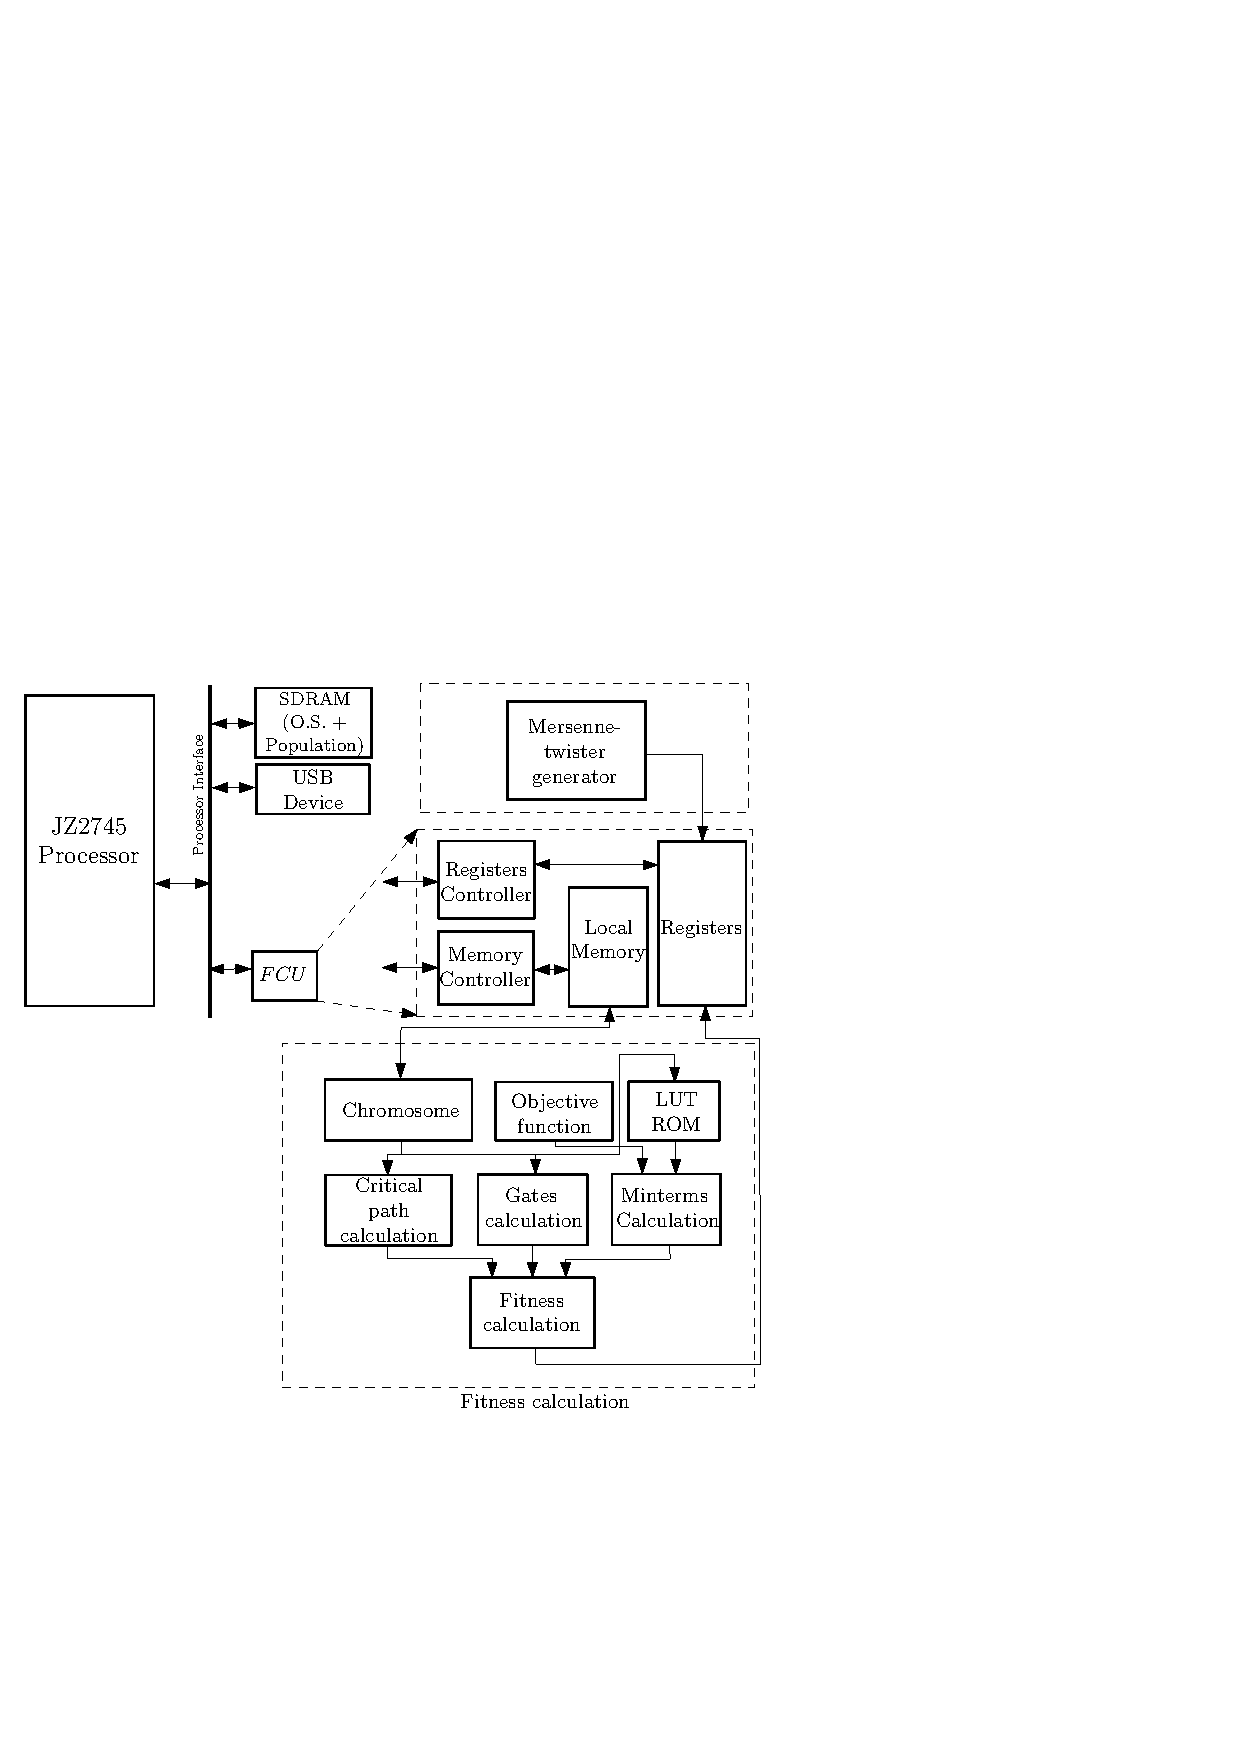
\includegraphics[width=7cm, height=6cm]{./images/hw_block_diagram_vertical} \end{center}
\caption{FCU structure.}\label{fig:hw_block}
\end{figure}



% &&&&&&&&&&&&&&&&&&&&&&&&&&&&&&&&&&&&&&&&&&&&&&&&&&&&&&&&&&&&&&&&&&&&&&&&&&&&&&&&&&&&&&&&&&&&&&&&&&&&
%                                                      EVALUACION
% &&&&&&&&&&&&&&&&&&&&&&&&&&&&&&&&&&&&&&&&&&&&&&&&&&&&&&&&&&&&&&&&&&&&&&&&&&&&&&&&&&&&&&&&&&&&&&&&&&&&
\section{Performance evaluation.}

SIE performance was compared to HPC and GPU. The HPC setup is made up of 18 eServer BladeCenters with 256 JS20 nodes (512 processors), using a Myrinet network with 1 Gbps bandwidth. The GPU architecture is based on a NVIDIA GTS450, made by 192 CUDA cores. The response time is measured in three scenarios: 1) number of input variables (4, 8 or 12, corresponding to a comparator problem of 2, 4 and 6 bits); 2) population size (512, 1024 or 2048) and 3) number of nodes running the experiment, ranged from 1 to 6 in SIE, and 2 to 16 or 64 in ALTAMIRA. The first and second parameters determine the size of the problem. 

\textbf{Response Time:}
Figure \ref{fig:rt_vars} shows the response time for both platforms with different numbers of nodes and variables with 1024 individuals during 100 generations. These results show the high performance of SIE cluster for the algorithm. This experiment demonstrates that the response time for SIE does not depend on the size of the problem. In contrast, response time in ALTAMIRA has a high dependency of the size of the problem, because individuals had to be evaluated by software. Figure \ref{fig:rt_indv} shows the response time in both architectures when varying the number of individuals of the population. It is observed that both architectures have a strong dependency of the number of individuals in the algorithm. This is because increasing this number causes an increment of the software computational load for both clusters. Even in this scenario, SIE shows an excellent performance compared to ALTAMIRA.

\begin{figure}[h!]
\begin{center}
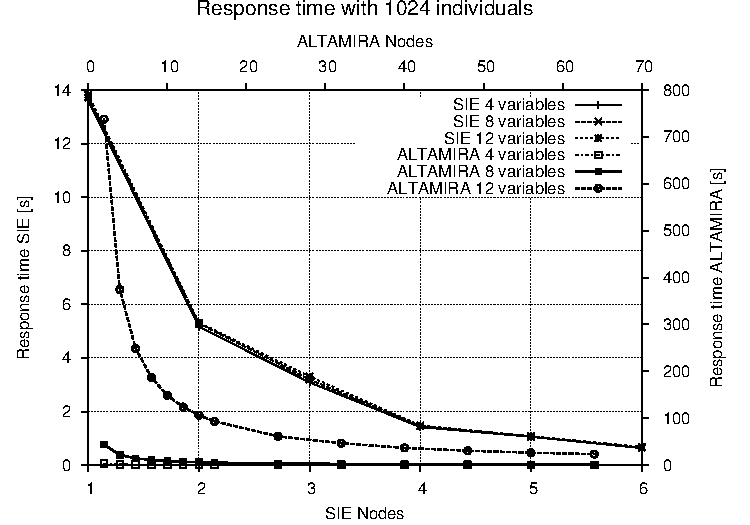
\includegraphics[width=7cm, height=4cm]{./images/response_time_1024indiv} 
\end{center}
\caption{Response time in SIE and ALTAMIRA for different number of variables.}
\label{fig:rt_vars}
\end{figure}

\begin{figure}[h!]
\begin{center} 
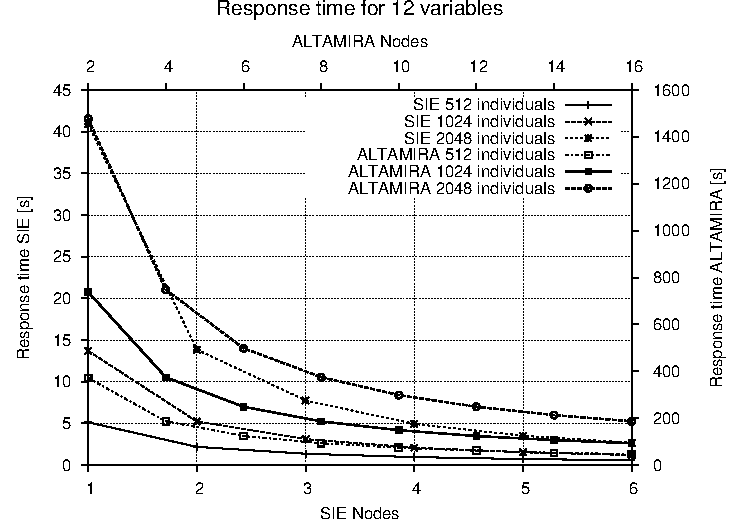
\includegraphics[width=7cm, height=4cm]{./images/response_time_12var} 
\end{center}
\caption{Response time in SIE and ALTAMIRA for different number of individuals.}
\label{fig:rt_indv}
\end{figure}
%%%%%%%%%%%%%%%%%%%%%

Figure \ref{fig:rt_indv2} shows the response time of executing the GP in the graphics hardware with problems of 4, 8 and 12 variables are fixed. Varying the number of islands and threads, can be observed that the best scenario is obtained when the number of threads is increased independently the number of islands. This is because when more threads are launched more parallelism is performed in the system, until the maximum of threads permitted by the GPUs is reached.


\begin{figure}[h!]
\begin{center} 
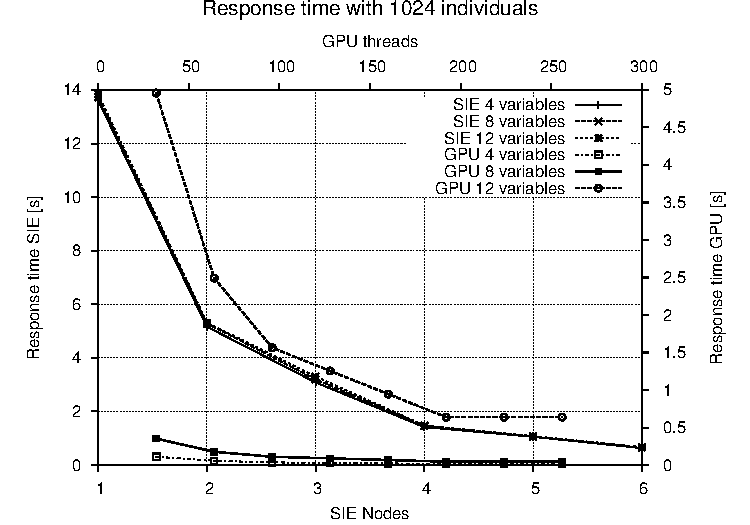
\includegraphics[width=8cm, height=4cm]{./images/response_time_1024indiv_gpu} 
\end{center}
\caption{Response time in SIE and GPU for different number of individuals.}
\label{fig:rt_indv2}
\end{figure}


The speedup of the SIE vs ALTAMIRA was up to 180 for 12-variable problems. The excellent performance of SIE can be explained because individuals have been directly tested in hardware (FPGA), obtaining a combination of their true table on each cycle of the system clock. On the other hand, individuals evaluated in software by ALTAMIRA require a lot of system clocks, causing response times hundreds of times higher than SIE.                                                  
On the other hand, the speedup number when SIE and GPU are compared was up to 2 for 12-variable problems. This can be explained because the whole population have been tested in hardware, obtaining a combination of their output on each cycle of the system clock. But, when an individual is tested in software, each combination requires a set of instructions, that requires a lot of cycles of the system clock.
In \cite{SEKANINA2008, ABYSEK2010} the obtained speedup is about 30-40 when 1 accelerator processor was used and compared against a single PC.

% &&&&&&&&&&&&&&&&&&&&&&&&&&&&&&&&&&&&&&&&&&&&&&&&&&&&&&&&&&&&&&&&&&&&&&&&&&&&&&&&&&&&&&&&&&&&&&&&&&&&
%                                                                     CONCLUSIONES Y TRABAJO FUTURO
% &&&&&&&&&&&&&&&&&&&&&&&&&&&&&&&&&&&&&&&&&&&&&&&&&&&&&&&&&&&&&&&&&&&&&&&&&&&&&&&&&&&&&&&&&&&&&&&&&&&&

\section{Conclusions and future work.}
This paper presented a novel way to evaluate individuals in an intrinsic evolvable algorithm on an open embedded platform called SIE, and results were compared to an HPC called ALTAMIRA and a high performance NVIDIA GPU. To accelerate the evolution process, a coprocessor was implemented to calculate the fitness function and to generate random numbers, improving the performance for problems with more than 6 bits. 

Results showed a speedup of 2 when SIE was compared to GPU, even when 192 processing cores were used in the last one. When compared with ALTAMIRA, SIE showed a speedup up to 180, due the high computational load in software when 16 nodes were used in ALTAMIRA. Significant speedup numbers were obtained due individuals have been directly tested in hardware, getting a combination of their true table on each cycle of the system clock. In the other hand, when an individual is tested in software, each combination requires a set of instructions, that requires a lot of cycles of the system clock.


Tests proved that the algorithm is more effective for 4-bit and 8-bit problems. 12-bit problems in SIE had excellent performance, but because the search space is too long, converging to a suitable solution was difficult for the algorithm. This problem could be solved as future work with some improvements in terms of multiple FCUs inside an FPGA, more nodes, and other hardware-accelerated genetic operators.



\bibliographystyle{plain}
\bibliography{./biblio_EHW.bib}

\end{document}
